\section{Duomenų bazė}
\label{sec:duomenu_baze}

OAuth antrajam faktoriui duomenų bazėje nereikia saugoti jokios paslapties -- pakanka susieti vartotoją su jo \textit{Google} identifikatoriumi \texttt{sub}. Siūloma schema pavaizduota \ref{fig:db_schema} pav., o lentelių laukai aprašyti \ref{tab:db_users}--\ref{tab:db_auth_events} lentelėse.

\begin{figure}[H]
    \centering
    \begin{adjustbox}{max width=\textwidth}
    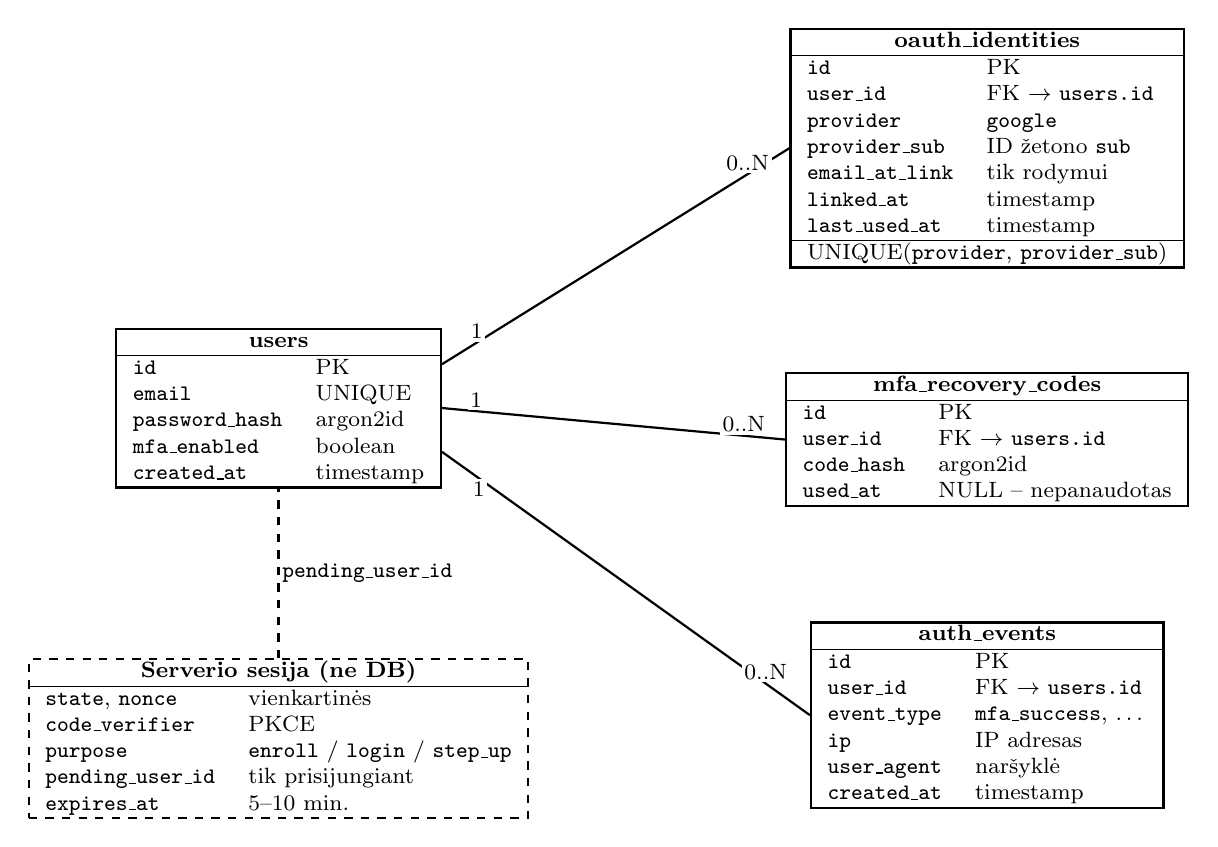
\begin{tikzpicture}[
        entity/.style={draw, thick, fill=white, inner sep=0pt, font=\footnotesize},
        session/.style={draw, thick, dashed, fill=white, inner sep=0pt, font=\footnotesize},
        rel/.style={thick},
        card/.style={font=\footnotesize, fill=white, inner sep=1pt},
    ]
        \node[entity] (users) at (0,0) {%
            \begin{tabular}{l l}
                \multicolumn{2}{c}{\textbf{users}} \\ \hline
                \texttt{id}             & PK \\
                \texttt{email}          & UNIQUE \\
                \texttt{password\_hash} & argon2id \\
                \texttt{mfa\_enabled}   & boolean \\
                \texttt{created\_at}    & timestamp \\
            \end{tabular}};

        \node[entity] (oauth) at (9,3.3) {%
            \begin{tabular}{l l}
                \multicolumn{2}{c}{\textbf{oauth\_identities}} \\ \hline
                \texttt{id}              & PK \\
                \texttt{user\_id}        & FK $\to$ \texttt{users.id} \\
                \texttt{provider}        & \texttt{google} \\
                \texttt{provider\_sub}   & ID žetono \texttt{sub} \\
                \texttt{email\_at\_link} & tik rodymui \\
                \texttt{linked\_at}      & timestamp \\
                \texttt{last\_used\_at}  & timestamp \\ \hline
                \multicolumn{2}{l}{UNIQUE(\texttt{provider}, \texttt{provider\_sub})} \\
            \end{tabular}};

        \node[entity] (codes) at (9,-0.4) {%
            \begin{tabular}{l l}
                \multicolumn{2}{c}{\textbf{mfa\_recovery\_codes}} \\ \hline
                \texttt{id}         & PK \\
                \texttt{user\_id}   & FK $\to$ \texttt{users.id} \\
                \texttt{code\_hash} & argon2id \\
                \texttt{used\_at}   & NULL -- nepanaudotas \\
            \end{tabular}};

        \node[entity] (events) at (9,-3.9) {%
            \begin{tabular}{l l}
                \multicolumn{2}{c}{\textbf{auth\_events}} \\ \hline
                \texttt{id}          & PK \\
                \texttt{user\_id}    & FK $\to$ \texttt{users.id} \\
                \texttt{event\_type} & \texttt{mfa\_success}, \ldots \\
                \texttt{ip}          & IP adresas \\
                \texttt{user\_agent} & naršyklė \\
                \texttt{created\_at} & timestamp \\
            \end{tabular}};

        \node[session] (sess) at (0,-4.2) {%
            \begin{tabular}{l l}
                \multicolumn{2}{c}{\textbf{Serverio sesija (ne DB)}} \\ \hline
                \texttt{state}, \texttt{nonce} & vienkartinės \\
                \texttt{code\_verifier}        & PKCE \\
                \texttt{purpose}               & \texttt{enroll} / \texttt{login} / \texttt{step\_up} \\
                \texttt{pending\_user\_id}     & tik prisijungiant \\
                \texttt{expires\_at}           & 5--10 min. \\
            \end{tabular}};

        \draw[rel] (users.15) -- node[card, pos=0.1, above] {1} node[card, pos=0.88, above] {0..N} (oauth.west);
        \draw[rel] (users.0) -- node[card, pos=0.1, above] {1} node[card, pos=0.88, above] {0..N} (codes.west);
        \draw[rel] (users.-15) -- node[card, pos=0.1, below] {1} node[card, pos=0.88, above] {0..N} (events.west);
        \draw[rel, dashed] (sess.north) -- node[card, right] {\texttt{pending\_user\_id}} (users.south);
    \end{tikzpicture}
    \end{adjustbox}
    \caption{Duomenų bazės schema ir laikini sesijos duomenys.}
    \label{fig:db_schema}
\end{figure}


\begin{table}[H]
    \centering
    \caption{Lentelė \texttt{users} (jau egzistuojanti, papildoma \texttt{mfa\_enabled} lauku).}
    \label{tab:db_users}
    \begin{tabularx}{\textwidth}{l l L}
        \toprule
        \textbf{Laukas} & \textbf{Tipas} & \textbf{Paskirtis} \\
        \midrule
        \texttt{id} & UUID, PK & Vartotojo identifikatorius \\
        \texttt{email} & TEXT, UNIQUE & Prisijungimo vardas \\
        \texttt{password\_hash} & TEXT & Slaptažodžio maiša (argon2id) -- pirmasis faktorius \\
        \texttt{mfa\_enabled} & BOOLEAN & Ar reikalauti antrojo faktoriaus \\
        \texttt{created\_at} & TIMESTAMP & Paskyros sukūrimo laikas \\
        \bottomrule
    \end{tabularx}
\end{table}

\begin{table}[H]
    \centering
    \caption{Lentelė \texttt{oauth\_identities} (vartotojo ir \textit{Google} paskyros susiejimas).}
    \label{tab:db_oauth}
    \begin{tabularx}{\textwidth}{l l L}
        \toprule
        \textbf{Laukas} & \textbf{Tipas} & \textbf{Paskirtis} \\
        \midrule
        \texttt{id} & UUID, PK & Įrašo identifikatorius \\
        \texttt{user\_id} & UUID, FK & Nuoroda į \texttt{users.id} \\
        \texttt{provider} & TEXT & Tapatybės teikėjas (\texttt{google}) \\
        \texttt{provider\_sub} & TEXT & ID žetono \texttt{sub}; pagal jį tikrinamas antrasis faktorius \\
        \texttt{email\_at\_link} & TEXT & \textit{Google} el. paštas susiejimo metu. Naudojamas tik rodymui, bet ne tikrinimui \\
        \texttt{linked\_at} & TIMESTAMP & Susiejimo laikas \\
        \texttt{last\_used\_at} & TIMESTAMP & Paskutinio sėkmingo patvirtinimo laikas \\
        \bottomrule
    \end{tabularx}
\end{table}

Lentelei \texttt{oauth\_identities} taikomi du unikalumo apribojimai. UNIQUE(\texttt{provider}, \texttt{provider\_sub}) užtikrina, kad viena \textit{Google} paskyra būtų susieta tik su viena mūsų sistemos paskyra. UNIQUE(\texttt{user\_id}, \texttt{provider}) leidžia vartotojui susieti tik vieną \textit{Google} paskyrą.

\begin{table}[H]
    \centering
    \caption{Lentelė \texttt{mfa\_recovery\_codes} (vienkartiniai atkūrimo kodai).}
    \label{tab:db_recovery}
    \begin{tabularx}{\textwidth}{l l L}
        \toprule
        \textbf{Laukas} & \textbf{Tipas} & \textbf{Paskirtis} \\
        \midrule
        \texttt{id} & UUID, PK & Įrašo identifikatorius \\
        \texttt{user\_id} & UUID, FK & Nuoroda į \texttt{users.id} \\
        \texttt{code\_hash} & TEXT & Atkūrimo kodo maiša (argon2id); pats kodas nesaugomas \\
        \texttt{used\_at} & TIMESTAMP, NULL & Panaudojimo laikas (NULL -- kodas dar nepanaudotas) \\
        \bottomrule
    \end{tabularx}
\end{table}

\begin{table}[H]
    \centering
    \caption{Lentelė \texttt{auth\_events} (autentifikavimo įvykių žurnalas).}
    \label{tab:db_auth_events}
    \begin{tabularx}{\textwidth}{l l L}
        \toprule
        \textbf{Laukas} & \textbf{Tipas} & \textbf{Paskirtis} \\
        \midrule
        \texttt{id} & UUID, PK & Įrašo identifikatorius \\
        \texttt{user\_id} & UUID, FK & Nuoroda į \texttt{users.id} \\
        \texttt{event\_type} & TEXT & \texttt{mfa\_enrolled}, \texttt{mfa\_success}, \texttt{mfa\_failed}, \texttt{mfa\_disabled}, \texttt{recovery\_used} \\
        \texttt{ip} & TEXT & IP adresas (vietai nurodyti pranešime vartotojui) \\
        \texttt{user\_agent} & TEXT & Naršyklė ir įrenginys \\
        \texttt{created\_at} & TIMESTAMP & Įvykio laikas \\
        \bottomrule
    \end{tabularx}
\end{table}

Jei taikomas rizika paremtas MFA (žr.~\ref{subsec:rizika} poskyrį), papildomai reikalinga lentelė \texttt{trusted\_devices}. Joje saugomi \texttt{user\_id}, slapuko maiša, naršyklė ir galiojimo pabaiga.

\textbf{Laikini duomenys (serverio sesija, ne duomenų bazė).} Vienam OAuth srautui reikalingos reikšmės saugomos serverio sesijoje:
\begin{itemize}
    \item \texttt{state}, \texttt{nonce}, \texttt{code\_verifier} -- vienkartinės atsitiktinės reikšmės;
    \item \texttt{purpose} -- srauto tikslas: \texttt{enroll}, \texttt{login} arba \texttt{step\_up};
    \item \texttt{pending\_user\_id} -- vartotojas, teisingai įvedęs slaptažodį (tik prisijungiant);
    \item \texttt{expires\_at} -- galiojimo pabaiga (5--10 min.).
\end{itemize}
Šios reikšmės ištrinamos iš karto po grįžimo iš \textit{Google}, nesvarbu, ar patvirtinimas pavyko.

\textbf{Kas nesaugoma.} Laikantis duomenų kiekio mažinimo principo~\cite{bdar}, nesaugomi:
\begin{itemize}
    \item \textit{Google} slaptažodis -- aplikacija jo niekada nemato;
    \item prieigos ir atnaujinimo (\textit{angl. refresh}) žetonai. Antrajam faktoriui jie nereikalingi, o jų saugojimas tik didintų riziką;
    \item visas ID žetonas -- pakanka jo \texttt{sub}.
\end{itemize}

\textbf{Konfigūracija.} \texttt{GOOGLE\_CLIENT\_ID}, \texttt{GOOGLE\_CLIENT\_SECRET} ir \texttt{REDIRECT\_URI} laikomi aplinkos kintamuosiuose arba slaptųjų duomenų saugykloje, ne duomenų bazėje. \texttt{client\_secret} niekada neturi patekti į naršyklę ar kodo repozitoriją.
